Wraz ze wzrostem świadomości użytkowników na temat cyberbezpieczeństwa wzrasta liczba podatności, które są wykrywane oraz ogłaszane między innymi w publicznych bazach wiedzy, takich jak Krajowa Baza Danych Podatności (ang. National Vulnerability Database, w skrócie NVD) \cite{booth2013national}. Od 2016 każdy kolejny rok uznawany jest za rekordowy ze względu na rosnącą liczbę wykrytych podatności. Przykładowo w pierwszej połowie 2020 roku ogłoszono około 9 799 nowych podatności dotyczących bezpieczeństwa sprzętu oraz oprogramowania, co - w porównaniu do tego samego okresu z roku 2019 - pozwala odnotować wzrost o 34\%. Dodatkowo z raportów organizacji monitorujących zagrożenia internetowe wynika, że jedną z przyczyn na tak znaczący wzrost liczby podatności, w stosunku do lat poprzednich, jest pandemia SARS-CoV-2 \cite{SkyboxR-2020}. Raport opublikowany przez firmę Skybox określa w swoim podsumowaniu rok 2020 jako rekordowy pod względem liczby wykrywania nowych typów zagrożeń. Wykryto dwa razy więcej wariantów Malware, odnotowano wzrost na poziomie 106\%  nowych rodzajów Ransomware oraz 128\% nowych rodzajów Trojana. Jak podaje raport, w samym 2020 roku tylko część ze zgłoszonych 18 341 nowych podatności będzie aktywnie wykorzystywana. Wszystkie wspomniane wcześniej informacje oznaczają ogromny wzrost danych dotyczących nowych podatności oraz wektorów ataków. Wzrost ten powoduje, że zespoły do spraw cyberbezpieczeństwa mierzą się z niezwykle trudnym zadaniem wykrycia najbardziej istotnych kwestii oraz przekierowania działań w obszary wymagające największego priorytetu \cite{SkyboxR-2021}.

\bigbreak
Wzrost liczby wykrywanych podatności przekłada się na bezpieczeństwo organizacji oraz jakość świadczonych przez nie usług \cite{walkowski2018impact}. Znane publicznie podatności, wykryte, lecz nienaprawione w infrastrukturze, mogą spowodować wielomilionowe straty czy też doprowadzić do całkowitego bankructwa. W tym celu, aby pomóc organizacjom, opracowano program zarządzania podatnościami, który służy jako ochronna warstwa przed zagrożeniami w wykrytych zabezpieczeniach.

\bigbreak
Niemniej jednak duży napływ informacji z różnych systemów bezpieczeństwa nie ułatwia administratorom pracy i stanowi wyzwanie dla wielu organizacji \cite{Gartner-2020}. Pierwszą kwestią związaną z zarządzaniem podatnościami jest upływ czasu między identyfikacją a eliminacją podatności. Jak wyjaśnia Gartner, „\emph{Większość organizacji kieruje się filozofią stopniowego zmniejszania ryzyka, z polityką zarządzania podatnościami i poprawkami koncentrującymi się na ograniczaniu i łataniu procentu luk w zabezpieczeniach w określonym czasie, na przykład naprawianie 90\% podatności o dużym znaczeniu w ciągu 2 tygodni od wykrycia. Ogranicza to zarządzanie podatnościami do czysto metrycznego ćwiczenia, w którym ryzyko jest wyrażone jako wartość liczbowa, którą można zmniejszyć.}”. Faktem jest, że potencjalny atakujący nie będzie skupiał się na naprawionych podatnościach, skupi się natomiast na pozostałych 10\%, które pozostają nienaprawione \cite{rochford2008t}.

\bigbreak
Haldar i Mishra pokazują w \cite{haldar2017mathematical} rangę czasu reakcji na nowo pojawiające się zagrożenia, a także podkreślają, jak bardzo znaczące jest szybkie ustalanie priorytetów i naprawianie podatności, aby zmaksymalizować wysiłek wymagany do przełamania zabezpieczeń. Ponadto w raporcie \cite{Gartner-2020} poruszone zostały inne kwestie mające wpływ na skuteczność programu zarządzania podatnościami, mianowicie:
\begin{itemize}
    \item brak możliwości natychmiastowego usunięcia wszystkich zidentyfikowanych podatności,
    \item proces zarządzania podatnościami nie jest możliwy bez skutecznej komunikacji,
    \item niewystarczające zasoby przeznaczone na naprawę spowodują kumulację podatności,
    \item naprawianie tylko „wysokich” i „krytycznych” podatności jest niewystarczające.
\end{itemize}

\bigbreak
Powyższe kwestie wynikają między innymi z faktu, że dostawcy komercyjnego oprogramowania, przykładowo \cite{beale2004nessus, fsecure2021, qualys2021, ibmxforce}, udostępniają własne metody priorytetyzacji podatności bez informowania użytkownika końcowego o szczegółach procesu podejmowania decyzji. Nieznajomość algorytmów ustalania priorytetów może niekorzystnie wpłynąć na proces naprawiania podatności. Jest to spowodowane faktem, że organizacje, korzystające z określonego rozwiązania, polegają na nieznanych algorytmach ustalania priorytetów, a co za tym idzie, nie mają one wpływu na decyzje przez nie podejmowane.

\bigbreak
Dalsza część rozprawy poświęcona jest procesowi zarządzania podatnościami z wykorzystaniem powszechnego systemu oceny podatności (ang. Common Vulnerability Scoring System, w skrócie CVSS). W kolejnych rozdziałach posłużono się skrótem pochodzącym z języka angielskiego CVSS, gdyż jest on ogólnie przyjęty w literaturze.

\section{Czym jest podatność?}
Aby zrozumieć koncepcję procesu zarządzania podatnościami, należy zacząć od poznania, czym jest podatność w systemie komputerowym oraz w jaki sposób jest oznaczana \cite{mann1999towards} i oceniana \cite{cvsspecification}.

\bigbreak
Według \cite{jukka2019look} podatność „\emph{to błędy w oprogramowaniu, które ujawniają słabości systemów komputerowych}”. W konsekwencji podatności w oprogramowaniu związane są bezpośrednio z procesem wytwarzania oprogramowania. Autorzy w \cite{morrison2018vulnerabilities} zwracają uwagę, że wykrywanie błędów, problemów i podatności w trakcie procesu tworzenia oprogramowania jest czasochłonne. Co więcej zgłaszane podatności często nie są wykrywane przez zespół programistów wytwarzających dane oprogramowanie, a pochodzą od niezależnych badaczy. 

\bigbreak
Duży wpływ na liczbę wykrywanych podatności przez niezależnych badaczy ma powszechny dostęp do Internetu oraz niejednokrotnie darmowych programów szkoleniowych z zakresu cyberbezpieczeństwa. Dodatkowym czynnikiem jest chęć zdobycia sławy oraz nagrody w coraz to liczniejszych programach typu ''nagroda za błąd'' (ang. Bug Bunty), w których uzyskanie realnego wynagrodzenia za wykryte błędy bezpieczeństwa staje się najważniejsze. Stawki wahają się od kilku do kilkunastu tysięcy, a w niektórych przypadkach nawet miliona dolarów. Przystąpienie do programu ''nagroda za błąd'' jest darmowe, dostępne dla każdego, co jeszcze bardziej zwiększa jego atrakcyjność \cite{malladi2019bug}. Istnieje też druga strona medalu, osoby, które w sposób nielegalny wyszukują podatności, wykorzystują je w celu szantażowania organizacji, pozyskania okupu czy też wyrządzenia szkód.
\FloatBarrier
%%%%%%%%%%%%%%%%%%%%%%%%%%%%%%%%%%%%%%%%%%%%%%%%

%%%%%%%%%%%%%%%%%%%%%%%%%%%%%%%%%%%%%%%%%%%%%%%%
\subsection{Metody oznaczania podatności}
Pomysł stworzenia Powszechnego Standardu Oznaczania Podatności (ang. Common Vulnerability Enumeration, w skrócie CVE) został przedstawiony w \cite{mann1999towards}. W kolejnych rozdziałach posłużono się skrótem pochodzącym z języka angielskiego CVE, ogólnie przyjętym w literaturze.

\bigbreak
Autorzy koncepcji CVE dostrzegli potrzebę wprowadzenia spójnego sposobu oznaczania podatności w celu usprawnienia komunikacji wewnętrznej w swojej organizacji. Każdy system bezpieczeństwa, który był przez nich używany i który próbowali zintegrować, posiadał swój własny sposób identyfikacji oraz nazewnictwa podatności \cite{mann1999towards, martin2001managing, fall2019common}. W rezultacie porównanie danych od różnych dostawców i powiązanie ich z innymi systemami bezpieczeństwa było bardzo czasochłonne \cite{mann1999towards, fall2019common}. Koncepcja powszechnego standardu oznaczania podatności została zaakceptowana przez branżę i literaturę do tego stopnia, że znalazła zastosowanie nie tylko w systemach wykrywania włamań (ang. Intrusion Detection System, w skrócie IDS) \cite{mell2003overview}, ale w każdej dziedzinie związanej z cyberbezpieczeństwem \cite{kaya2019study, food2016postmarket, wang2018mining}. Ponadto, od 1999 r. wielu producentów oprogramowania i organizacji non-profit opracowywało, promowało i wdrażało różnorodne konkurujące ze sobą systemy oceny podatności, przykładowo: X-Force \cite{ibmxforce}, Symantec \cite{broadcom-2020}, Microsoft \cite{msrc-2020}, Redhat \cite{Redhat-2020}, Mozilla \cite{mozilla-2020}, Secunia \cite{secunia-2020}, Vulpen  \cite{liu2012improving}, Google \cite{chromium-2020}, VRSS \cite{liu2012improving} oraz CVSS \cite{mell2006common}. W chwili obecnej \cite{ibmxforce, broadcom-2020, msrc-2020, Redhat-2020, mozilla-2020, chromium-2020} nadal utrzymują swoje działy badawcze, mimo to wspierają rozwiązanie \cite{mell2006common}. Rozwiązanie \cite{secunia-2020} nie jest już rozwijane, natomiast \cite{liu2012improving} nie przyjęło się.

\bigbreak
CVSS został po raz pierwszy wprowadzony jako projekt badawczy przez Krajową Radę Doradczą ds. Infrastruktury USA (ang. National Infrastructure Advisory Council, w skrócie NIAC) w 2005 r. \cite{mell2006common}, a następnie przyjęty przez inne organizacje. Wersje CVSS 2.0 i CVSS 3.1 \cite{cvs2005specification, cvs2019specification} są podzielone na trzy kategorie: bazową (ang. Base), czasową (ang. Temporal) i środowiskową (ang. Environmental).

\bigbreak
Kategoria bazowa reprezentuje właściwości podatności, którą uważa się za niezmienną w czasie. Natomiast w rzeczywistości może ulec ona zmianie, jeśli na jaw wyjdą informacje wymagające aktualizacji oceny. W stworzonym oprogramowaniu zaimplementowano mechanizm aktualizacji kategorii bazowej dla wszystkich podatności. Mechanizm został opisany w rozdziale drugim.

\bigbreak
Właściwości kategorii bazowej obejmują złożoność dostępu, wektor dostępu oraz ocenę stopnia, w jakim podatność zagraża poufności, integralności i dostępności systemu. Kategoria czasowa opisuje właściwości, które mogą się zmieniać w czasie. W szczególności odnosi się do istnienia publicznego exploita oraz dostępności poprawek. Charakterystyka czasowa była badana w szczególności przez Ruohonena w \cite{cvsspecification}, podczas gdy dla charakterystyki środowiskowej \cite{mell2003overview} naukowcy starali się wyrazić ryzyko wartości, potencjalną stratę i rozpowszechnienie dotkniętych systemów w rozważanym środowisku.

\bigbreak
Oba standardy CVSS 2.0 oraz CVSS 3.x nadal są szeroko wykorzystywane przez operatorów sieci teleinformatycznych, ponieważ nie wszystkie wcześniej wykryte podatności zostały przeliczone do nowego standardu CVSS \cite{fall2019common}. Dlatego w niniejszej pracy wykorzystane zostały oba standardy CVSS. Autor rozprawy za pomocą opracowanego oprogramowania dodatkowo wspiera badania dotyczące wykorzystania mechanizmów uczenia maszynowego, które pozwalają na przeliczanie standardu CVSS 2.0 do CVSS 3.x. Wyniki opublikowane zostały w pracach \cite{Nowak-cldd-2021, Nowa2109Conversion}.

\FloatBarrier
%%%%%%%%%%%%%%%%%%%%%%%%%%%%%%%%%%%%%%%%%%%%%%%%

%%%%%%%%%%%%%%%%%%%%%%%%%%%%%%%%%%%%%%%%%%%%%%%%
\subsection{Wprowadzenie do standardu CVSS 2.0}
\label{sec:cvss_2_standard}
Standard CVSS 2.0 został zaprezentowany w 2007 roku. Organizacje takie jak Risk Based Security oraz Open Security Foundation opublikowały otwarty list dotyczący wad i błędów związanych z CVSS 2.0 \cite{eiram2013cvssv2}. Autorzy przytoczyli brak szczegółowości w metrykach, co skutkowało wynikami, które nie pozwalają odpowiednio rozróżnić typu podatności i profilu ryzyka. Zauważono również, że system punktacji CVSS wymaga zbyt dużej wiedzy na temat dokładnego wpływu podatności. Pomimo wykazanych wad standardu CVSS, jest on wykorzystywany do dzisiaj.

\bigbreak
W niniejszej pracy wykorzystano metryki opisane w dokumencie „\emph{A Complete Guide to the Common Vulnerability Scoring System Version 2.0}” \cite{cvs2005specification}, skupiając się na wzorach pozwalających na obliczenie oceny środowiskowej. Aby tego dokonać, ważne jest zrozumienie, w jaki sposób obliczana jest wartość oceny bazowej ($B_S$). Wartości poszczególnych oznaczeń wykorzystanych w równaniu opisane zostały w Tabeli \ref{tab:chapter1:cvss_2_property}. Kategoria krytyczności podatności jest przydzielana wg Tabeli \ref{tab:cvss_criticality_2} i wynika bezpośrednio z wartości oceny bazowej ($B_S$).

\begin{equation}
    B_S = round\_to\_1\_decimal(((0.6* I)  +(0.4*E)-1.5)* f(I))
\end{equation}

Gdzie:
\begin{equation}
    I=10.41 * (1 - (1 - C_I) * (1 - I_I) * (1 - A_I))
\end{equation}

\begin{equation}
    E=20 * A_V * A_C * A_U
\end{equation}

\begin{equation}
f(I) = 
\begin{cases}
0,\text{jeżeli I=0} \\
0.176\text{ w innym przypadku} \\
\end{cases}
\end{equation}

\begin{table}[tbh]
\caption{Wartości cech CVSS 2.0 Base.}
\begin{center}
\label{tab:chapter1:cvss_2_property}
\begin{tabular}{cllc}
\hline \noalign {\smallskip}
\textbf{Oznaczenie} & \textbf{Znaczenie} & \textbf{Wartość metryczna} & \textbf{Wartość liczbowa} \\
\hline \noalign {\smallskip}
$C_I$ & Wpływ na poufność         & None          & 0.000 \\
      & (ang. Confidentiality Impact)  & Partial       & 0.275 \\
$I_I$ & Wpływ na integralność     & Complete      & 0.660 \\
      & (ang. Integrity Impact)        &               &       \\
$A_I$ & Wpływ na dostępność       &               &       \\
      & (ang. Availability Impact)     &               &       \\
\hline \noalign {\smallskip}
$A_V$ & Wektor dostępu            & Local access & 0.395 \\
      & (ang. Access Vector)           & Adjacent network accesible & 0.646 \\
      &                           & Network accessible & 1.00 \\
\hline \noalign {\smallskip}
$A_C$ & Złożoność dostępu         & High     & 0.350 \\
      & (ang. Access Complexity)       & Medium	 & 0.610 \\
      &                           & Low	     & 0.710 \\
\hline \noalign {\smallskip}
$A_U$ & Wymagane poświadczenie  & Multiple instances & 0.450 \\
      & (ang. Authentication)        & Single instance & 0.560 \\
	  &                         & No authentication & 0.704 \\
\hline \noalign {\smallskip}

\end{tabular}
\end{center}
\end{table}

\bigbreak
Końcowe obliczanie oceny środowiskowej ($E_S$) dokonywane jest na podstawie poniższego wzoru (znaczenie poszczególnych oznaczeń opisano w Tabeli \ref{tab:chapter1:cvss_2_property_env}):

\begin{equation}
\label{eq:cvss2_es}
E_S=round\_to\_1\_decimal((T+ (10 - T) * C_D) * T_D)
\end{equation}

Gdzie:

\begin{equation}
T=min(10, 10.41 * (1 - (1 - C_I * C_R) * (1 - I_I * I_R) * (1- A_I * A_R))
\end{equation}


\begin{table}[tbh]
\caption{Wartości cech CVSS 2.0 Environmental.}
\label{tab:chapter1:cvss_2_property_env}
\begin{center}
\begin{tabular}{cllc}
\hline \noalign {\smallskip}
\textbf{Oznaczenie} & \textbf{Znaczenie} & \textbf{Wartość metryczna} & \textbf{Wartość liczbowa} \\
\hline \noalign {\smallskip}
$C_R$ & Wymóg poufności                  & Low & 0.50\\
      & (ang. Confidentiality Requirement)    & Medium & 1.00 \\
$I_R$ & Wymóg integralności              & High & 1.51 \\
      & (ang. Integrity Requirement)          & Not defined & 1.00 \\
$A_R$ & Wymóg dostępności & & \\
      & (ang. Availability Impact) & & \\
\hline \noalign {\smallskip}
$CDP$ & Potencjalne szkody dodatkowe    & None	& 0.00 \\
      & (ang. Collateral Damage Potential)   & Low	& 0.10 \\
      &                                 & Low – Medium & 0.30 \\
      &                                 & Medium-High  & 0.40 \\
      &                                 & High	& 0.50 \\
      &                                 & Not defined & 	0.00 \\

\hline \noalign {\smallskip}
$TD$ & Dystrybucja podatności          & None	      & 0.00 \\
      & (ang. Target Distribution)           & Low	      & 0.25 \\
      &                                 & Medium	  & 0.75 \\
      &                                 & High	      & 1.00 \\
      &                                 & Not defined & 1,00 \\
\hline \noalign {\smallskip}

\end{tabular}
\end{center}
\end{table}

\begin{table}[tbh]
\caption{Zakres ocen oraz opis według CVSS 2.0 w przekładzie na krytyczność podatności.}
\begin{center}
\label{tab:cvss_criticality_2}
\begin{tabular}{lll}
\hline \noalign {\smallskip}
\textbf{Zakres} & \textbf{Kategoria} & \textbf{Opis} \\
\hline \noalign {\smallskip}
0.0 – 3.9  & Niska	    & Potencjalny atakujący może być w stanie zebrać wrażliwe    \\
           &            & informacje o infrastrukturze, takie jak np. wersje        \\
           &            & zainstalowanego oprogramowania. Posiadając te informacje  \\
           &            & może stosunkowo łatwo znaleźć podatności                  \\
           &            & dot. konkretnych wersji oprogramowania i próbować         \\
           &            & je wykorzystać. Podatności o klasyfikacji niskiej         \\
           &            & należy wyeliminować przy kolejnej konserwacji środowiska. \\
\hline 
4.0 – 6.9  & Średnia    & Podatności mogą prowadzić do wykorzystania aplikacji lub \\
           &            & serwera przez potencjalnego atakującego w sposób niezgodny \\
           &            & z przeznaczeniem. Podatności o klasyfikacji średniej \\
           &            & należy naprawić w dogodnym momencie, ale nie należy z nimi \\
           &            & zwlekać. \\
\hline 
7.0 – 10.0 & Wysoka	    & Potencjalny atakujący może przejąć kontrolę nad            \\
           &            & serwerem/aplikacją lub istnieje poważny wyciek wrażliwych  \\
           &            & danych. Podatności o klasyfikacji wysokiej powinny zostać \\
           &            & naprawione tak szybko, jak to możliwe. \\
\hline \noalign {\smallskip}
\end{tabular}
\end{center}
\end{table}

\newpage
Aby każda obliczona ocena była zrozumiała przez odbiorcę, zapisywana jest także w postaci wektorowej. Przykładową postać zapisano poniżej, znaczenie poszczególnych parametrów opisano w Tabeli \ref{tab:chapter1:cvss_2_vector}.

\begin{equation}
\label{eq:chapter1:cvss_2_en_vector}
AV:N/AC:M/Au:N/C:P/I:P/A:P/CDP:L/TD:H/CR:L/IR:L/AR:L
\end{equation}

\begin{table}[tbh]
\caption{Możliwe wartości wektora CVSS 2.0.}
\begin{center}
\label{tab:chapter1:cvss_2_vector}
\begin{tabular}{clc}
\hline \noalign {\smallskip}
\textbf{Oznaczenie} & \textbf{Znaczenie} & \textbf{Możliwe wartości} \\
\hline \noalign {\smallskip}
AV & Wektor dostępu  & L, A, N \\
   & (ang. Access Vector) &        \\

\hline \noalign {\smallskip}
AC & Złożoność dostępu   &  H, M, L \\
   & (ang. Access Complexity) & \\

\hline \noalign {\smallskip}
C &  Wpływ na poufność       & N, P, C \\
  & (ang. Confidentiality Impact) & \\
I & Wpływ na integralność    & \\
  & (ang. Integrity Impact)       & \\ 
A & Wpływ na dostępność      & \\
  & (ang. Availability Impact)    & \\

\hline \noalign {\smallskip}
CDP	& Potencjalne szkody dodatkowe & N, L, LM, MH, H, ND \\
    & (ang. Collateral Damage Potential) & \\

\hline \noalign {\smallskip}
TD & Dystrybucja podatności & 	N, L, M, H, ND \\
   & (ang. Target Distribution)  & \\

\hline \noalign {\smallskip}
CR & Wymóg poufności               & N, P, C \\
   & (ang. Confidentiality Requirement) & \\
IR & Wymóg integralności           & \\
   & (ang. Integrity Impact)            & \\
AR & Wymóg dostępności             & \\
   & (ang. Availability Impact)         & \\

\hline \noalign {\smallskip}
\end{tabular}
\end{center}
\end{table}

\bigbreak
Na szczególną uwagę zasługują parametry równania, takie jak dystrybucja podatności (ang Target Disribution, w skrócie $TD$) oraz potencjalne szkody dodatkowe (ang. Collateral Damage Potential, w skrócie $CDP$). Pierwszy wspomniany parametr $TD$ służy ustaleniu liczby systemów wrażliwych na daną podatność i jest on specyficzny dla badanego środowiska. Parametr $CDP$ odpowiedzialny jest za określenie poziomu strat. Im wyższa wartość parametru $CDP$, tym wyższe potencjalne straty dla całego środowiska teleinformatycznego wynikające z wykorzystania danej podatności. Dokładna propozycja automatycznego określenia wartości obu parametrów została opisana w rozdziale drugim. Wpływ wszystkich parametrów środowiskowych na ocenę bazową został opisany w rozdziale czwartym oraz piątym.

\FloatBarrier
%%%%%%%%%%%%%%%%%%%%%%%%%%%%%%%%%%%%%%%%%%%%%%%%

%%%%%%%%%%%%%%%%%%%%%%%%%%%%%%%%%%%%%%%%%%%%%%%%
\subsection{Wprowadzenie do standardu CVSS 3.x}
\label{sec:cvss_3_standard}
Standard CVSS 3.0 jako aktualizacja standardu 2.0 został zaprezentowany w 2015 roku. Wprowadza on nowy sposób obliczania podatności oraz wyklucza parametry $TD$ i $CDP$. Oba parametry prawdopodobnie zostaną przywrócone w wersji 4 standardu \cite{cvs2021improvements}, lecz na chwilę obecną poziom prac jeszcze nie jest na tyle zaawansowany, aby można go było brać pod uwagę.

\bigbreak
Wersja CVSS 3.0 odbiega od swojego poprzednika sposobem wyznaczania kategorii podatności oraz przydzielaniem cech wektorów dla składowej oceny. Trzy podstawowe kategorie przedstawione na początku rozdziału bazowa, czasowa i środowiskowa zostały zachowane. W kategorii bazowej wprowadzono takie zmiany, jak:
\begin{itemize}
    \item w miarach dotyczących poufności, integralności zmieniono parametry na: \emph{brak, niski} lub \emph{wysoki},
    \item do wektora ataku została dodana wartość fizyczna (ang. Physical, w skrócie $P$), która wskazuje lukę w zabezpieczeniach, w której atakujący musi mieć fizyczny dostęp do systemu, aby móc ją wykorzystać,
    \item dodano nowy parametr interakcja z użytkownikiem (ang. User Interaction, w skrócie $UI$). Parametr ten wskazuje, czy do wykorzystania podatności atakującemu potrzebna jest interakcja z użytkownikiem,
    \item dodano nowy parametr w postaci wymaganych uprawnień (ang. Privileges Required, w skrócie $PR$), celem wskazania, czy atakujący musi posiadać jakiekolwiek uprawnienia (np. administracyjne), aby pomyślnie móc wykorzystać podatność.
\end{itemize}

\bigbreak
W kategorii środowiskowej największą zmianą jest zastąpienie parametrów $TD$ oraz $CDP$ na tak zwane zmodyfikowane wyniki bazowe. Zasadniczo każda z metryk bazowych może zostać zmodyfikowana przez organizację, aby odzwierciedlić różnice w swoim środowisku teleinformatycznym. Wynika to z faktu, że organizacja, mimo korzystania z otwartego i powszechnego standardu CVSS, zmuszona jest monitorować ryzyka w sposób subiektywny przez pryzmat swojego środowiska teleinformatycznego.

\bigbreak
Po ukazaniu się standardu CVSS 3.0 wiele firm skrytykowało go za niedokładne opisanie wartości parametrów, pozwalających na ich różną interpretację. W 2019 roku wydano aktualizacje CVSS 3.1, która skonkretyzowała opis metryk, tworząc je bardziej zrozumiałe dla odbiorcy, sam sposób obliczania oceny podatności, postać parametrów i reprezentacja wektora nie uległy zmianie.

\bigbreak
W niniejszej pracy posłużono się metrykami opisanymi w dokumencie „\emph{Common Vulnerability Scoring System v3.1: Specification Document}” \cite{cvs2019specification}, skupiając się na wzorach pozwalających na obliczenie oceny środowiskowej ($E_S$). Wartość parametrów wykorzystanych w równaniach opisana została w Tabeli \ref{tab:wstep:cvss_3}. Krytyczność podatności wynikająca z pozyskanej oceny, przydzielana jest według Tabeli \ref{tab:cvss_criticality_3}.

\begin{equation}
E_S = 
\begin{cases}
0, \text{jeżeli} f(M) \leq 0 \\
min(f(M) + E, 10)\text{, jeżeli S = U} \\
min(1.08 * (f(M) + E), 10)\text{, w innym przypadku} \\
\end{cases}
\end{equation}

Gdzie:
\begin{equation}
f(M) = 
\begin{cases}
6.42 * M\text{,jeżeli S = Niezmieniony} \\
7.52 * (M - 2.029) - 3.25 * (M * 0. 9731)^{13} \\
\end{cases}
\end{equation}

\begin{equation}
M = min(1 - [(1 - C_R * C_I) * (1 - I_R * I_I) * (1 - A_R * A_I)], 0.915)
\end{equation}

\begin{equation}
E=8.22 * AV * AC *PR * UI
\end{equation}

\begin{table}[tbh]
\caption{Wartości cech CVSS 3.x Environmental.}
\label{tab:wstep:cvss_3}
\begin{center}
\begin{tabular}{cllc}
\hline \noalign {\smallskip}
\textbf{Oznaczenie} & \textbf{Znaczenie} & \textbf{Wartość metryczna} & \textbf{Wartość liczbowa} \\
\hline \noalign {\smallskip}
$C_I$ & Wpływ na poufność         & High      & 0.56 \\
      & (ang. Confidentiality Impact)  & Low       & 0.22 \\
$I_I$ & Wpływ na integralność     & None      & 0    \\
      & (ang. Integrity Impact)        &           &      \\
$A_I$ & Wpływ na dostępność       &           &      \\
      & (ang. Availability Impact)     &           &      \\
\hline \noalign {\smallskip}
$A_V$ & Wektor ataku              & Network  & 0.85  \\
      & (ang. Attack Vector)           & Adjacent & 0.62  \\
      &                           & Local    & 0.55  \\
      &                           & Physical & 0.2   \\
\hline \noalign {\smallskip}
$A_C$ & Złożoność ataku           & High     & 0.44 \\
      & (ang. Attack Complexity)       & Low	     & 0.77 \\

\hline \noalign {\smallskip}
$P_R$ & Wymagane uprawnienia    &  High & 0,45 \\
      & (ang. Privileges Required)	&  Low	& 0,56 \\
	  &                         &  None	& 0.85 \\

\hline \noalign {\smallskip}
$U_I$ & Interakcja z użytkownikiem & Required & 0.62 \\
      &                            &          & (lub 0.68, \\
      &                            &          & jeśli S = Required) \\
      & (ang. User Interaction)         & None & 0.85 \\
      &                            &      & (lub 0.68, \\
      &                            &      & jeśli S = Required) \\

\hline \noalign {\smallskip}
$C_R$ & Wymóg poufności               & Low	    & 0.50 \\
      & (ang. Confidentiality Requirement) & Medium	& 1.00 \\
$I_R$ & Wymóg integralności           & High	& 1.50 \\
      & (ang. Integrity Impact)            & Not defined	& 1.00\\
$A_R$ & Wymóg dostępności & \\
      & (ang. Availability Impact) & \\ 
\hline \noalign {\smallskip}

\end{tabular}
\end{center}
\end{table}


\begin{table}[tbh]
\caption{Zakres ocen według CVSS 3.x w przekładzie na krytyczność podatności.}
\begin{center}
\label{tab:cvss_criticality_3}
\begin{tabular}{lll}
\hline \noalign {\smallskip}
\textbf{Zakres} & \textbf{Kategoria} & \textbf{Opis} \\
\hline \noalign {\smallskip}
0.0        & Informacyjna & Potencjalny atakujący może zebrać podstawowe informacje    \\
           &              & o komputerze lub aplikacji (otwarte porty, serwisy, itd.)  \\
           &              & oraz może na ich podstawie wnioskować kolejne podatności.  \\
           &              & Należy naprawić podatności przy kolejnej większej          \\
           &              & rekonfiguracji środowiska. Podatności mają niewielki wpływ \\
           &              & na poziom bezpieczeństwa. \\
\hline
0.1 – 3.9  & Niska        & Potencjalny atakujący może być w stanie zebrać wrażliwe    \\
           &              & informacje o maszynie lub aplikacji, takie jak np.         \\
           &              & wersje zainstalowanego oprogramowania. Posiadając te       \\
           &              & informacje, może stosunkowo łatwo znaleźć podatności dot.   \\
           &              & konkretnych wersji oprogramowania i próbować je            \\
           &              & wykorzystać. Podatności należy naprawić przy kolejnej      \\
           &              & konserwacji środowiska. \\
\hline
4.0 – 6.9  & Średnia      & Podatności mogą prowadzić do wykorzystania aplikacji lub \\
           &              & serwera przez potencjalnego atakującego w sposób niezgodny \\ 
           &              & z przeznaczeniem systemu. Podatności należy naprawić \\
           &              & w dogodnym momencie, ale nie należy z nimi \\
           &              & zwlekać. \\
\hline
7.0 – 8.0  & Wysoka       & Potencjalny atakujący może przejąć kontrolę nad serwerem, \\
           &              & aplikacją lub istnieje poważny wyciek wrażliwych danych. \\
           &              & Podatności powinny zostać naprawione tak szybko, jak to   \\
           &              & możliwe.\\
\hline
8.1 – 10.0 & Krytyczna    & Atakujący może w łatwy sposób przejąć kontrolę nad maszyną, \\ 
           &              & aplikacją lub siecią. \\
           &              & Podatności wymagają natychmiastowej reakcji.\\
\hline \noalign {\smallskip}
\end{tabular}
\end{center}
\end{table}

\bigbreak
Tak jak w przypadku CVSS 2.0, w wersji CVSS 3.x również podawany jest całościowy wektor, którego przykładową postać zapisano poniżej. Znaczenie poszczególnych parametrów opisano w Tabeli \ref{tab:chapter1:cvss_vector_3}.

\begin{equation}
\label{eq:chapter1:cvss_2_vector}
AV:N/AC:H/PR:L/UI:R/S:U/C:L/I:L/A:L/CR:M/IR:L/AR:H
\end{equation}

\begin{table}[tbh]
\caption{Możliwe wartości wektora CVSS 3.x.}
\begin{center}
\label{tab:chapter1:cvss_vector_3}
\begin{tabular}{clc}
\hline \noalign {\smallskip}
\textbf{Oznaczenie} & \textbf{Znaczenie} & \textbf{Możliwe wartości} \\
\hline \noalign {\smallskip}
AV & Wektor ataku  & N, A, L, P \\
   & (ang. Attack Vector) &          \\

\hline \noalign {\smallskip}
AC & Złożoność ataku   &  L, H \\
   & (ang. Attack  Complexity) & \\

\hline \noalign {\smallskip}
Au & Wymagane poświadczenie   & M, S, N \\
   & (ang. Authentication) & \\

\hline \noalign {\smallskip}
S & Zakres   & U, C \\
   & (ang. Scope) & \\

\hline \noalign {\smallskip}
C &  Wpływ na poufność       & L, M, N, H \\
  & (ang. Confidentiality Impact) & \\
I & Wpływ na integralność    & \\
  & (ang. Integrity Impact)       & \\ 
A & Wpływ na dostępność      & \\
  & (ang. Availability Impact)    & \\

\hline \noalign {\smallskip}
PR & Wymagane uprawnienia  & H, L, N \\
   & (ang. Privileges Required) & \\

\hline \noalign {\smallskip}
UI & Interakcja z użytkownikiem  & R, N \\
   & (ang. User Interaction) & \\

\hline \noalign {\smallskip}
CR & Wymóg poufności               & L, M, N, H \\
   & (ang. Confidentiality Requirement) & \\
IR & Wymóg integralności           & \\
   & (ang. Integrity Impact)            & \\
AR & Wymóg dostępności             & \\
   & (ang. Availability Impact)         & \\

\hline \noalign {\smallskip}
\end{tabular}
\end{center}
\end{table}

\FloatBarrier
%%%%%%%%%%%%%%%%%%%%%%%%%%%%%%%%%%%%%%%%%%%%%%%%

%%%%%%%%%%%%%%%%%%%%%%%%%%%%%%%%%%%%%%%%%%%%%%%%
\section{Proces zarządzania podatnościami}
\label{sec:proces-zarzadzania-podatnosciami}
Obecne sieci korporacyjne składają się z tysięcy urządzeń oraz aplikacji, które obejmują różnorodne podmioty, począwszy od sieci biurowych, systemów finansowych i kadrowych po wyspecjalizowane konfiguracje, takie jak sterowanie procesem produkcyjnym, uzbrojeniem, systemem telekomunikacyjnym lub kontrolą środowiska \cite{al2019risk}, bez których procesy biznesowe mogą nie działać lub ich chwilowa niedostępność spowoduje potencjalnie wysokie straty \cite{nyanchama2005enterprise}. Jednym z dowodów na poparcie powyższej tezy, jest podatność o numerze CVE-2017-0143 nazwana przez badaczy jako Eternalblue \cite{cve-2017-0143}. Przy jej użyciu hakerzy stworzyli ransomware WannaCry, czyli złośliwe oprogramowanie, które w krótkim czasie zaszyfrowało bezpowrotnie tysiące terabajtów danych i spowodowało straty finansowe w korporacjach, takich jak Nissan czy FedEx \cite{mohurle2017brief, chen2017automated}, jeszcze bardziej uwypuklając potrzebę odpowiedniej implementacji procesu zarządzania podatnościami.

\bigbreak
W dojrzałych organizacjach proces zarządzania podatnościami pozwala na utrzymywanie ryzyka związanego z wykorzystaniem znanych podatności na najniższym możliwym poziomie \cite{walkowski2019container}. Głównym jego celem jest monitorowanie i identyfikacja nowych zagrożeń (w sprzęcie lub oprogramowaniu), które mogą wpłynąć na poufność, integralność lub dostępność zasobów IT organizacji. Proces zarządzania podatnościami jest również centralnym punktem gromadzenia i zatwierdzania wyjątków od naprawiania podatności, np. jeśli podatności nie można naprawić z powodu ograniczeń lub wgrana aktualizacja spowoduje, że kluczowe usługi staną się niedostępne.

\bigbreak
Proces zarządzania podatnościami jest procesem ciągłym, powtarzanym każdorazowo po zakończeniu poprzedniego cyklu. Wszystkie fazy procesu wskazane na rysunku \ref{fig:vm-cycle} zostały opisane w niniejszym rozdziale, w kolejności ich występowania. Cykliczność procesu wynika z faktu, że codziennie pojawiają się nowe zagrożenia, infrastruktura jest dynamiczna, nowo wprowadzona konfiguracja dla urządzenia sieciowego może wprowadzić nową podatność, więc po jednym, a nawet kilku zakończonych cyklach, organizacja nie może jednoznacznie stwierdzić, że zakończyła proces z sukcesem.

\bigbreak
W celu podniesienia skuteczności procesu, \cite{Gartner-2020} proponuję wprowadzenie w organizacji następujących stanowisk oraz odpowiedzialności:
\begin{itemize}
    \item szef bezpieczeństwa - osoba odpowiedzialna między innymi za proces zarządzania podatnościami w organizacji,
    \item inżynier ds. bezpieczeństwa - osoba odpowiedzialna za przeprowadzanie skanów zgodnie z procesem,
    \item właściciel zasobu - osoba odpowiedzialna za zasoby IT, które są skanowane w procesie; ponadto od właściciela zasobu zależy, czy podatność zostanie naprawiona, czy też ryzyko z nią związane zostanie zaakceptowane, najczęściej jest to osoba powiązana z biznesem,
    \item administrator zasobu - osoba odpowiedzialna za wdrażanie zaleceń, które powstały w wyniku przeprowadzonych skanów oraz procesu zarządzania podatnościami.
\end{itemize}

\begin{figure}[!ht]
\centering
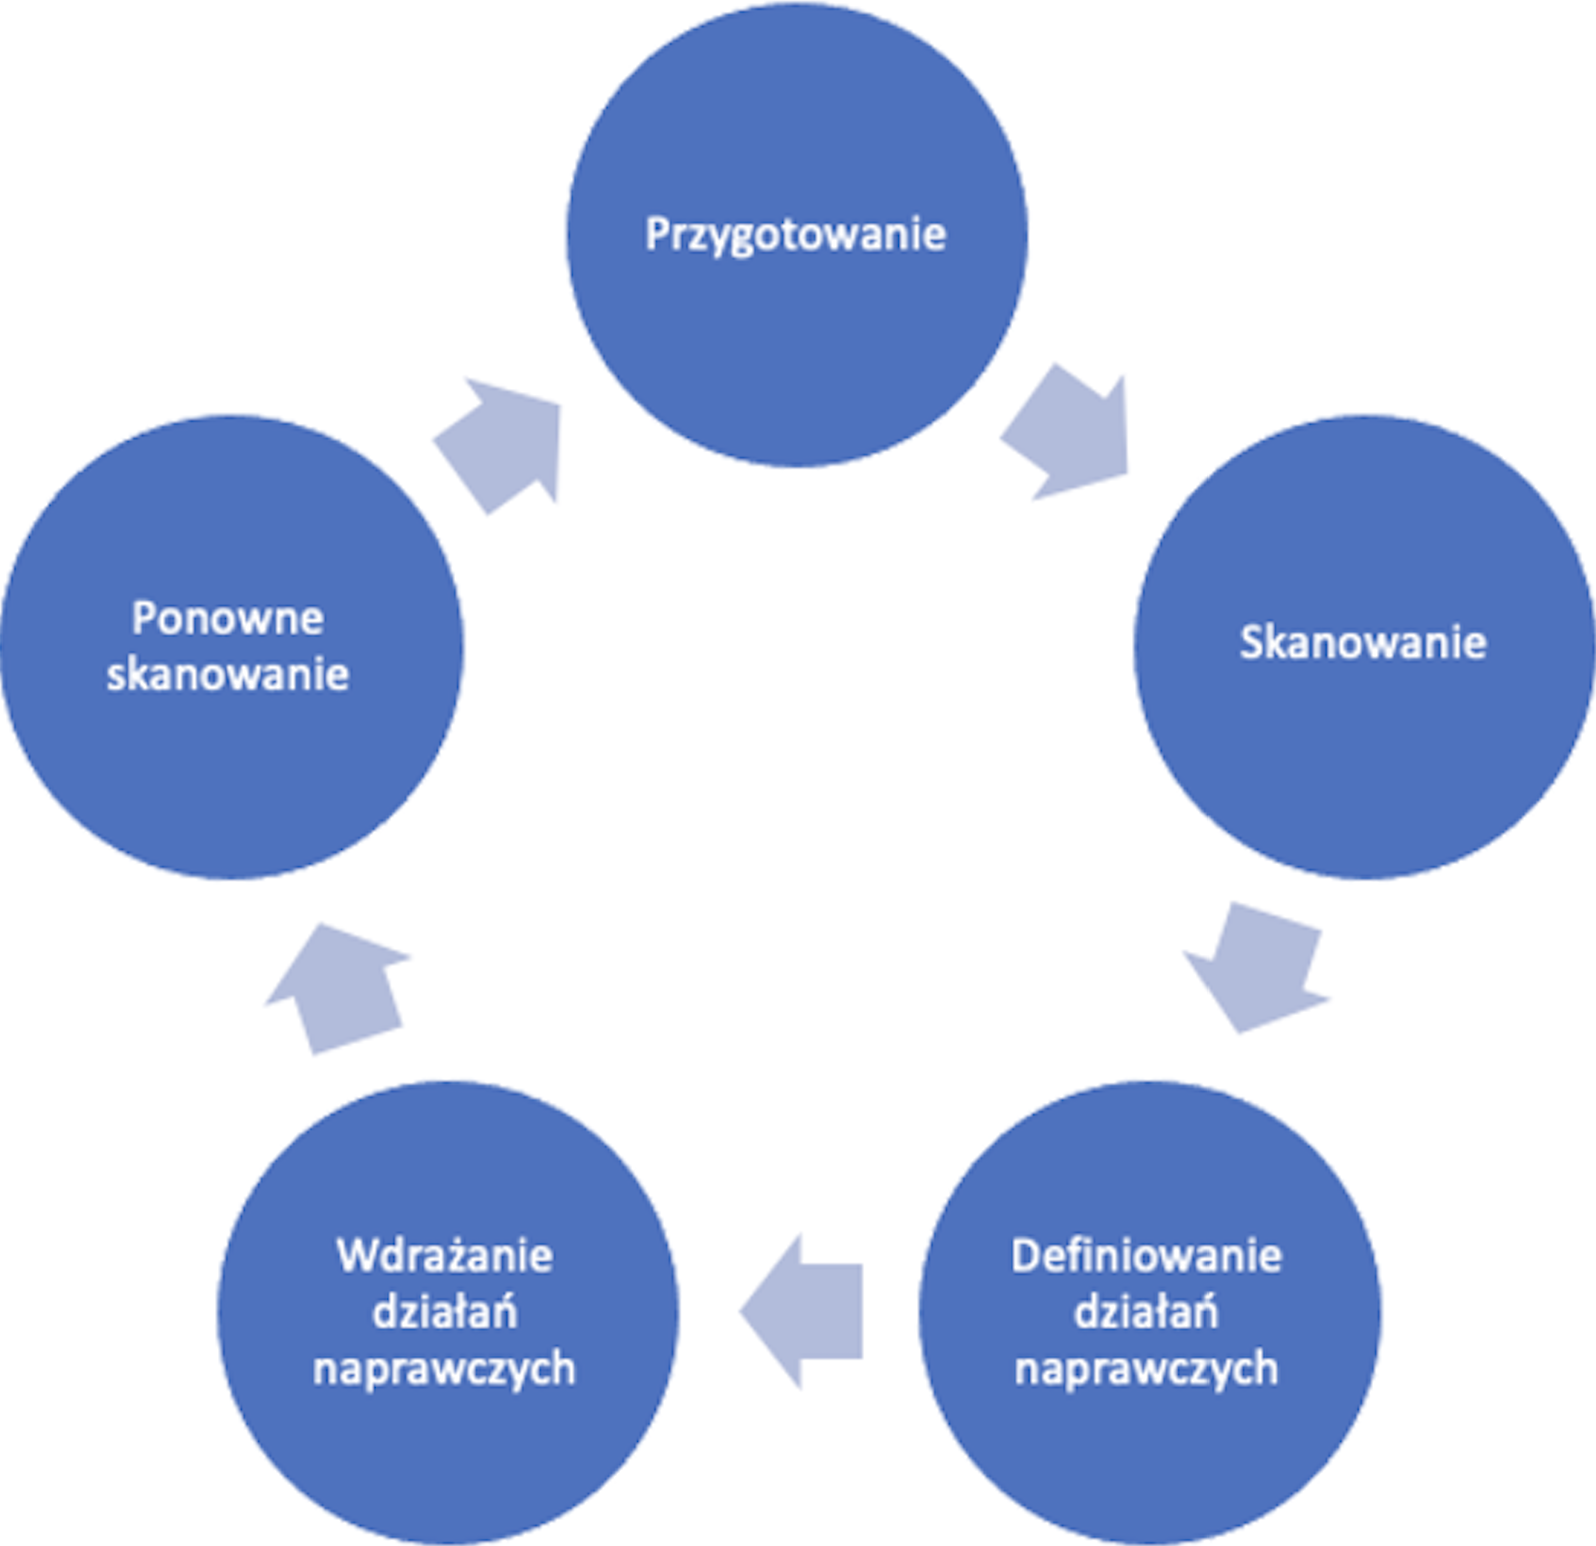
\includegraphics[width=.8\textwidth]{Chapters/Wstep/p-vm/cykl-vm.png}
\caption{Cykl procesu zarządzania podatnościami}
\label{fig:vm-cycle}
\end{figure}

%%%%%%%%%%%%%%%%%%%%%%%%%%%%%%%%%%%%%%%%%%%%%%%%

%%%%%%%%%%%%%%%%%%%%%%%%%%%%%%%%%%%%%%%%%%%%%%%%
\subsection{Przygotowanie}
W pierwszej fazie, przygotowawczej, najważniejsza jest inwentaryzacja zasobów, zapoznanie się ze środowiskiem sieciowym oraz posiadaną infrastrukturą. Po dokonaniu inwentaryzacji oraz zebraniu informacji na temat wykorzystywanego oprogramowania oraz sprzętu dla wszystkich zinwentaryzowanych zasobów nadawane są priorytety, dzięki którym możliwe będzie obliczenie potencjalnego ryzyka oraz podjęcie decyzji, które są kluczowe dla funkcjonowania organizacji.

\bigbreak
Po przeprowadzeniu inwentaryzacji osoba odpowiedzialna za proces, czyli szef bezpieczeństwa, definiuje zakres skanowania, następnie informuje właścicieli oraz administratorów zasobów o planowanym skanowaniu. Każde skanowanie może doprowadzić do obciążenia sieci lub systemów skanowanych, dlatego ważne jest, aby wyznaczyć odpowiednie okno czasowe, dzięki któremu odbywające się skanowanie będzie miało możliwie jak najmniejsze negatywne skutki dla funkcjonowanie skanowanych systemów (Rysunek \ref{fig:vm-prepare}).

\begin{figure}[!ht]
\centering
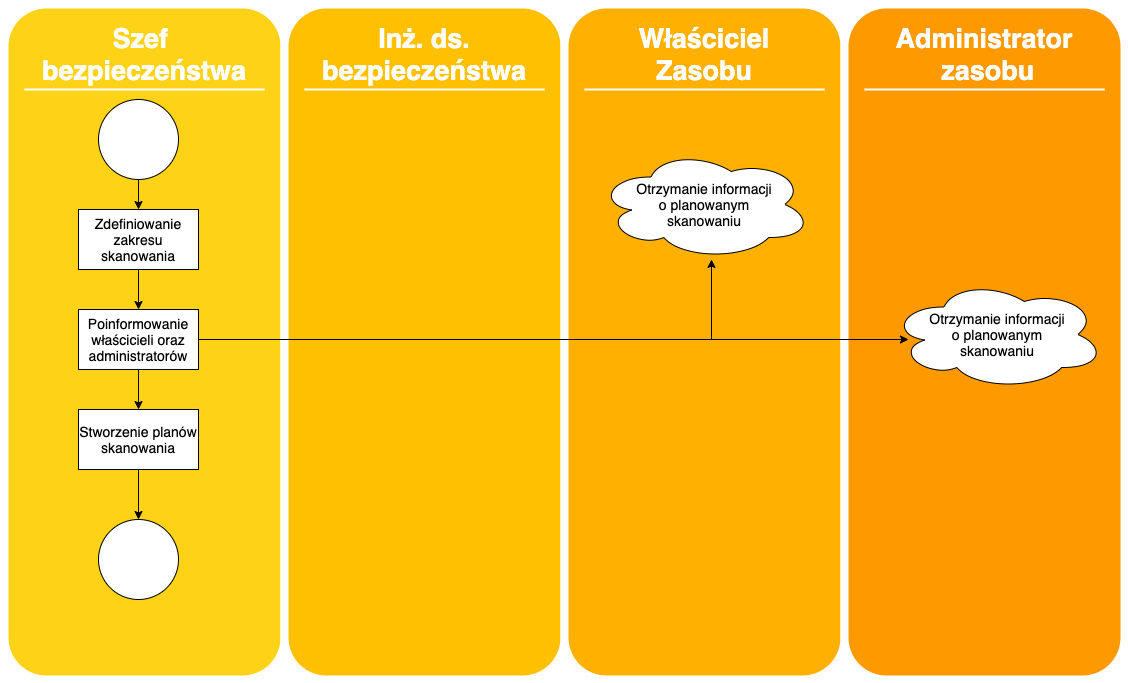
\includegraphics[width=.9\textwidth]{Chapters/Wstep/p-vm/vm-init.png}
\caption{Przepływ informacji w fazie planowania.}
\label{fig:vm-prepare}
\end{figure}
\FloatBarrier

%%%%%%%%%%%%%%%%%%%%%%%%%%%%%%%%%%%%%%%%%%%%%%%%

%%%%%%%%%%%%%%%%%%%%%%%%%%%%%%%%%%%%%%%%%%%%%%%%
\subsection{Skanowanie}
W fazie skanowania zasoby wybrane oraz zinwentaryzowane w fazie przygotowawczej są skanowane przez inż. ds. bezpieczeństwa za pomocą skanera podatności. Duży wpływ na jakość wyników ma zastosowane narzędzie oraz doświadczenie osoby wykonującej skany. W tym czasie również administratorzy zasobów powinni monitorować stabilność swoich systemów. W przypadku wykrycia problemów podczas skanowania administratorzy muszą zgłaszać je do osób wykonujących skanowanie. Wyniki oraz potencjalne problemy dostarczane są do wszystkich osób zaangażowanych w proces zarządzania podatnościami (Rysunek \ref{fig:vm-scanning}).

\begin{figure}[!ht]
\centering
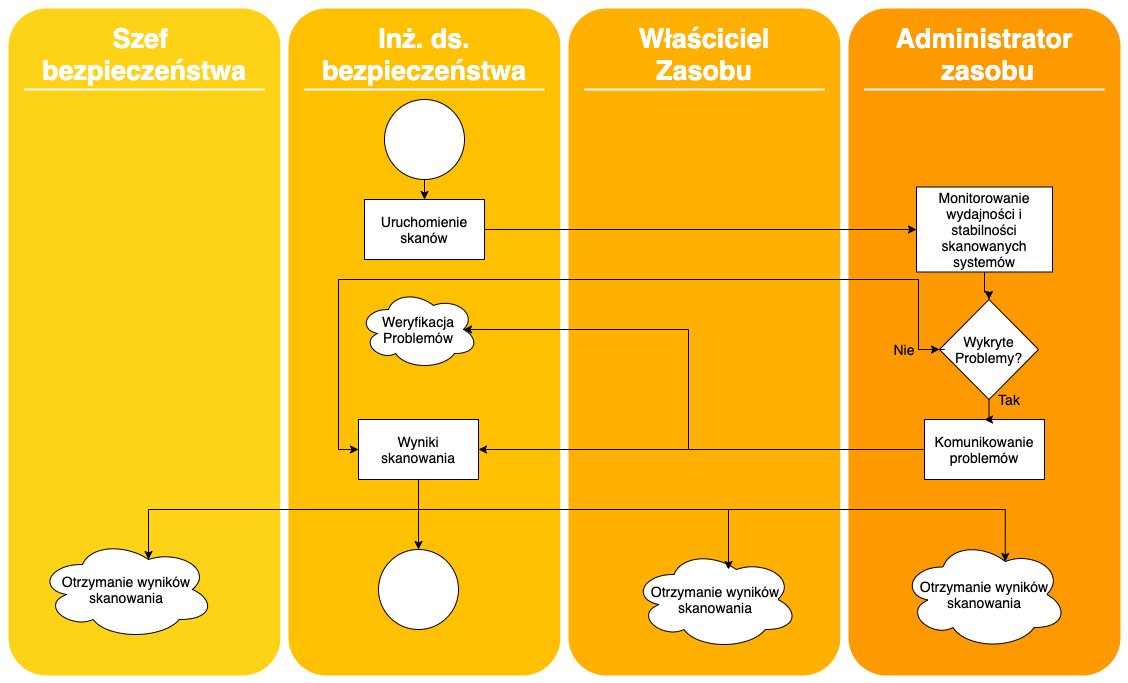
\includegraphics[width=.9\textwidth]{Chapters/Wstep/p-vm/scaninng.png}
\caption{Przepływ informacji w fazie skanowania.}
\label{fig:vm-scanning}
\end{figure}
\FloatBarrier
%%%%%%%%%%%%%%%%%%%%%%%%%%%%%%%%%%%%%%%%%%%%%%%%

%%%%%%%%%%%%%%%%%%%%%%%%%%%%%%%%%%%%%%%%%%%%%%%%
\subsection{Definiowanie działań naprawczych}
W fazie definiowania działań naprawczych zarówno inż. ds. bezpieczeństwa, jak i administrator zasobu powinni przeanalizować wynik skanowania podatności. Po przeprowadzeniu analiz przekazują wnioski i rekomendacje właścicielowi zasobu. Po otrzymaniu wszystkich informacji właściciel zasobu decyduje, czy ryzyko związanie z wykorzystaniem wykrytych podatności jest akceptowalne. Jeśli nie, powinien zdefiniować działania naprawcze. Jeżeli jednak zaakceptuje ryzyko, musi przekazać te informacje do szefa działu bezpieczeństwa w celu rozpoczęcia formalnego procesu akceptacji ryzyka. Nawet bez decyzji o podjęciu działań naprawczych należy zachować odpowiednią dokumentację na wypadek wzrostu ryzyka w przyszłości (Rysunek \ref{fig:vm-fixing}).

\begin{figure}[!ht]
\centering
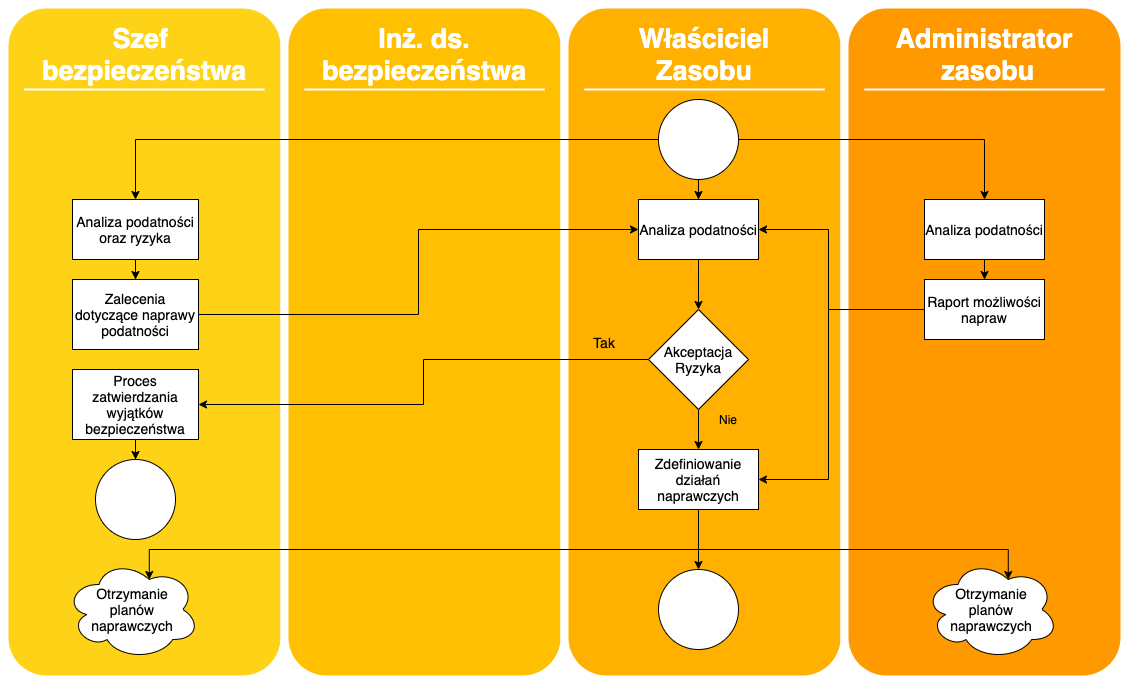
\includegraphics[width=.9\textwidth]{Chapters/Wstep/p-vm/vm-fixing.png}
\caption{Przepływ informacji w fazie definiowania działań naprawczych.}
\label{fig:vm-fixing}
\end{figure}
%%%%%%%%%%%%%%%%%%%%%%%%%%%%%%%%%%%%%%%%%%%%%%%%

%%%%%%%%%%%%%%%%%%%%%%%%%%%%%%%%%%%%%%%%%%%%%%%%
\subsection{Wdrażanie działań naprawczych}
W wielu przypadkach działania łagodzące są łatwiejsze do wdrożenia niż działania naprawcze, jednocześnie zapewniają już wystarczającą ochronę. Poprzez działania łagodzące rozumiemy wykorzystanie firewalli, systemów wykrywania włamań (ang. Intrusion Detection System, w skrócie IPS) lub zapory aplikacji internetowej (ang. Web Application Firewall, w skrócie WAF) – w zależności od dostępnego budżetu oraz zapotrzebowania. Metody łagodzące zamiast naprawy stosowane są w sytuacjach, w których naprawa jest zbyt kosztowna lub zachodzi wysokie ryzyko, że naprawa danej podatności może uszkodzić działanie systemów, przykładowo wgranie nowej wersji oprogramowania spowoduje destabilizację serwera – warto posiadać linię testową, aby przed udostępnieniem poprawki w środowisku produkcyjnym zbadać jak będzie się zachowywał zaktualizowany system. Po wykonaniu wszystkich działań naprawczych administrator powinien poinformować szefa bezpieczeństwa w celu umożliwienia rozpoczęcia kolejnej fazy procesu (Rysunek \ref{fig:flow-fixing}).

\begin{figure}[!ht]
\centering
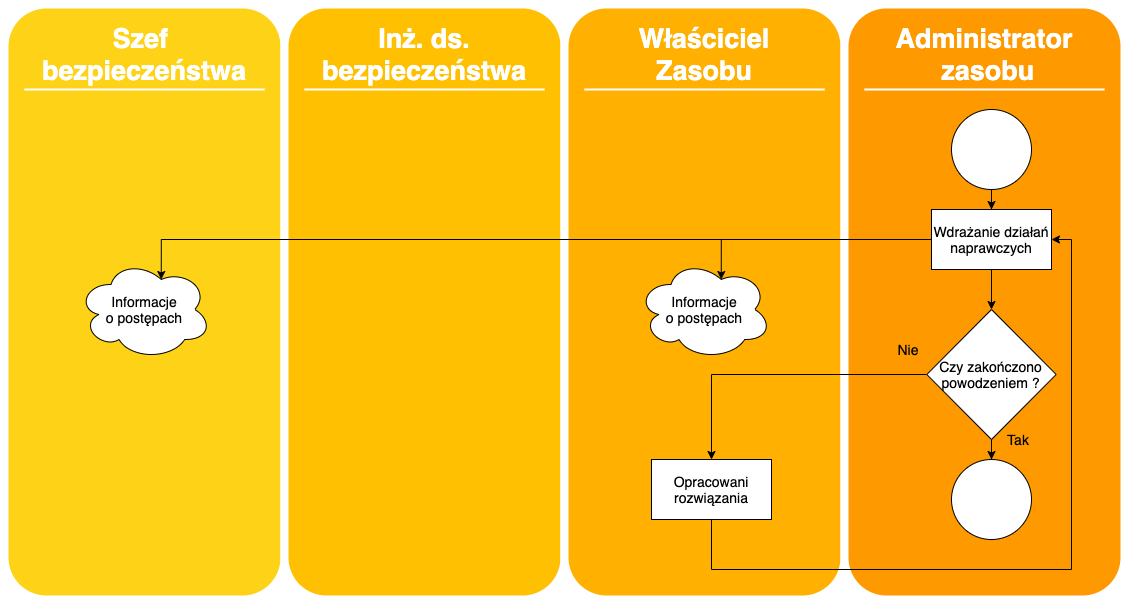
\includegraphics[width=.9\textwidth]{Chapters/Wstep/p-vm/flow-fixing.png}
\caption{Przepływ informacji w fazie wdrażania działań naprawczych.}
\label{fig:flow-fixing}
\end{figure}

%%%%%%%%%%%%%%%%%%%%%%%%%%%%%%%%%%%%%%%%%%%%%%%%

%%%%%%%%%%%%%%%%%%%%%%%%%%%%%%%%%%%%%%%%%%%%%%%%
\subsection{Ponowne skanowanie}
Ostatnia faza polega na uruchomieniu ponownego skanowania przez inżyniera ds. bezpieczeństwa, przeanalizowaniu uzyskanych wyników, a następnie poinformowaniu właściciela zasobu i szefa bezpieczeństwa. Szef bezpieczeństwa ocenia, czy działania naprawcze zakończyły się powodzeniem. W zależności od przyjętej koncepcji fazę tę można potraktować jako rozpoczęcie nowego cyklu życia procesu zarządzania podatnościami (Rysunek \ref{fig:rescan-flow}).
\begin{figure}[!ht]
\centering
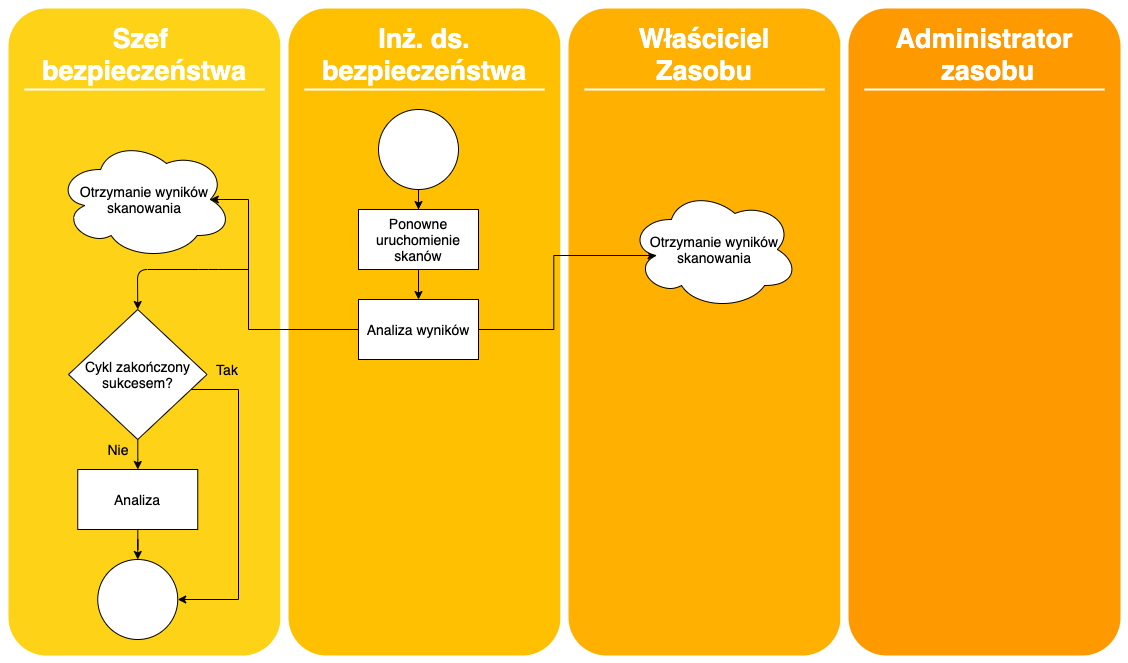
\includegraphics[width=.9\textwidth]{Chapters/Wstep/p-vm/rescan-flow.png}
\caption{Przepływ informacji w fazie ponownego skanowania.}
\label{fig:rescan-flow}
\end{figure}

%%%%%%%%%%%%%%%%%%%%%%%%%%%%%%%%%%%%%%%%%%%%%%%%

%%%%%%%%%%%%%%%%%%%%%%%%%%%%%%%%%%%%%%%%%%%%%%%%
\subsection{Podsumowanie}
Wdrażając proces zarządzania podatnościami, opisany w niniejszym rozdziale, dla każdej organizacji należy rozpocząć od fazy przygotowawczej, która jest najważniejsza. To właśnie w niej zostanie dokonana inwentaryzacja zasobów. Nie jest możliwe wdrożenie procesu, który ma poprawiać bezpieczeństwo organizacji oraz chronić przed zagrożeniami bez wiedzy, co powinno być chronione i na jakim poziomie. Kolejnym krokiem, który musi zostać wykonany, to wyszczególnienie zakresu odpowiedzialności dla wszystkich osób biorących udział w procesie. Ilość osób zaangażowanych w proces zarządzania podatnościami zależy od rozmiaru oraz kontekstu organizacji. Dla małej organizacji zakresy obowiązków zostaną zwiększone, przykładowo właściciel organizacji będzie pełnić funkcje szefa bezpieczeństwa oraz właściciela zasobu, natomiast pracownik będzie inż. ds. bezpieczeństwa oraz administratorem zasobu. Niemniej jednak proces zarządzania podatnościami będzie wyglądał tak samo. Nigdy nie powinno doprowadzać się do tego, aby jedna osoba była odpowiedzialna za wszystkie cztery zakresy odpowiedzialności, ponieważ nigdy nie będzie ona dość obiektywna w podejmowaniu decyzji dotyczącej ryzyka lub naprawy podatności. W dużej organizacji, w której dostępna jest większa liczba pracowników, zwiększy się ilość osób biorących udział w procesie, dzięki czemu zakres odpowiedzialności poszczególnych osób jest ściśle określony.

\bigbreak
W zależności od narzędzi wykorzystywanych oraz przyjętych ram czasowych dotyczących obsługi otrzymanego zgłoszenia w organizacji (ang. Service Level Agreement, w skrócie SLA) finalny czas naprawy podatności będzie się znacząco różnił. Zysk z wykorzystania proponowanego modelu zarządzania podatnościami w każdym przypadku będzie znaczący, a szacunkowa liczba roboczogodzin przedstawiona w rozdziale \ref{sec:modele-ewaluacji-efektywnosci} dla modelu zarządzania podatnościami pozwala na przyjęcie założeń dotyczących planowania czasochłonności oraz liczby zadań potrzebnych do wykonania zgodnie z nowoczesnym modelem pracy, jakim jest Agile \cite{alqudah2016review}. Rolą osób zarządzających zespołami jest zatrudnienie odpowiedniej liczby osób, tak aby pojedynczy pracownik nie stał się tak zwanym wąskim gardłem dla całego procesu zarządzania podatnościami. Na przykład zatrudnienie trzech pracowników może pozwolić na skrócenie liczby wymaganych roboczogodzin trzykrotnie. 

%%%%%%%%%%%%%%%%%%%%%%%%%%%%%%%%%%%%%%%%%%%%%%%%

%%%%%%%%%%%%%%%%%%%%%%%%%%%%%%%%%%%%%%%%%%%%%%%%
\section{Modele zarządzania podatnościami}
\label{sec:modele-zarzadzaia-podatnosciami}
Autorzy w pracach \cite{fruhwirth2009improving, ali2011software} podkreślą fakt, że w celu prawidłowego nadania priorytetu podatności organizacje powinny w ustandaryzowany sposób rozważyć wagę aktywów i ocenę podatności. Problem priorytetyzacji podatności jest od dawna omawiany w dostępnej literaturze \cite{chen2007stakeholder, eschelbeck2005laws, lai2007using, rieke2006modelling}. Większość organizacji o ugruntowanej pozycji, które poważnie traktują cyberbezpieczeństwo, ma wdrożony w mniejszym lub większym stopniu proces zarządzania podatnościami \cite{Gartner-2020, chen2007stakeholder, fruhwirth2009improving}. Jednak, jak zauważono w \cite{Gartner-2020, chen2007stakeholder, eschelbeck2005laws, lai2007using, rieke2006modelling}, każda organizacja podchodzi do problemu inaczej. Rozwiązania wymienione w raporcie \cite{Gartner-vm}, F-Secure \cite{fsecure2021}, Qualys \cite{qualys2021}, Rapid7 \cite{rapid72021} czy Tenable \cite{tenablevm2021} z jednej strony pomagają organizacjom przezwyciężyć problem zarządzania podatnościami, ale z drugiej mają dwie wady. Mianowicie są bardzo drogie i nie informują użytkowników o szczegółach procedury priorytetyzacji podatności. Na przykład Qualys używa 7-punktowej skali \cite{qualys2021}, Rapid7 przeprowadza priorytetyzację w zakresie od 1 do 1000 \cite{rapid72021}, natomiast Tenable nazwał swoją metodę priorytetyzacji VPR, dla której podane poziomy mieszczą się w zakresie od 1 do 10 \cite{tenablevm2021}.

\bigbreak
Oprócz rozwiązań komercyjnych w literaturze można znaleźć inne rozwiązania, takie jak: PatchRank \cite{yadav2019patchrank}, SecureRank \cite{miura2007securerank}, Vulcon \cite{farris2018vulcon}, CMS \cite{weintraub2016security}, czy VEST \cite{chen2019vest}. Rozwiązanie PatchRank skupia się wyłącznie na priorytetyzacji aktualizacji dla systemów SCADA \cite{yadav2019patchrank}. SecureRank wykorzystuje topologię sieci i potencjalną interakcję między serwerami do obliczenia ryzyka \cite{miura2007securerank}. Strategia oprogramowania Vulcon opiera się na dwóch elementarnych wskaźnikach: czasie pojawienia się podatności i całkowitym czasie ekspozycji na podatność \cite{farris2018vulcon} w cyklach miesięcznych. CMS skupia się na wykrywaniu podatności na podstawie korelacji bazy zasobów z bazą NVD, w związku z czym istnieje duże prawdopodobieństwo zgłaszania przez narzędzie podatności, które rzeczywiście nie istnieją lub pomijanie tych, które naprawdę znajdują się w środowisku \cite{weintraub2016security}. VEST natomiast skupia się na przewidywaniu jak szybko podatność może zostać wykorzystana przez atakującego \cite{chen2019vest}. Inne rozwiązania, np. \cite{yadav2019patchrank, miura2007securerank, farris2018vulcon, chen2019vest} nie uwzględniają wag zasobów i nie są dostosowane do rosnącej ilości danych w środowisku chmury obliczeniowej, przez co nie mogą być stosowane w każdej infrastrukturze sieciowej. Dodatkowo żadne z przedstawionych rozwiązań nie oferuje jednocześnie priorytetów dla CVSS 2.0 i CVSS 3.x. Wynika to z faktu, że nie wszystkie podatności zostały przekonwertowane z CVSS 2.0 do CVSS 3.x, mimo że CVSS 3.x lepiej ocenia istotę podatności i skuteczniej szacuje zagrożenia \cite{fall2019common, Nowak-cldd-2021, Nowa2109Conversion}.

\begin{figure}[!ht]
\centering
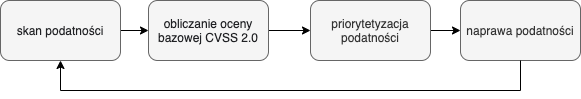
\includegraphics[width=.9\textwidth]{Chapters/Wstep/vm-models/vm-model-cvss2.png}
\caption{Model przepływu informacji w procesie zarządzania podatnościami z wykorzystaniem oceny bazowej CVSS 2.0.}
\label{fig:chapter1:vm-model-cvss2}
\end{figure}

\bigbreak
Wszystkie przedstawione wcześniej rozwiązania nie obejmują priorytetyzacji wykrytych podatności według oceny środowiskowej, przez co proces zarządzania podatnościami odbywa się z wykorzystaniem ocen bazowych. Rysunki \ref{fig:chapter1:vm-model-cvss2} i \ref{fig:chapter1:vm-model-cvss3} przestawiają modele procesu zarządzania podatnościami z wykorzystaniem ocen bazowych CVSS, w którym to wyniki otrzymane bezpośrednio ze skanera są prioretyzowane, a następnie przekazywane do administratorów zasobów w celu wykonania prac naprawczych. Na dodatkową uwagę zasługuje również fakt, że organizacje wspierają się metrykami zaproponowanymi przez Center for Internet Security (CIS), które powstały w 2010 roku \cite{CIS-2010, Walk2109-Automatic} w celu mierzenia stanu bezpieczeństwa infrastruktury teleinformatycznej. Organizacje, aby spełnić wymagania stawiane przez metryki CIS, najczęściej wybierają standard oparty na ocenie bazowej CVSS 2.0 (Rysunek \ref{fig:chapter1:vm-model-cvss2}), pomijając model \ref{fig:chapter1:vm-model-cvss3} z uwagi na wcześniej wspomnianą wadę CVSS 3.x dotyczącą braku oceny bazowej dla wszystkich podatności.


\begin{figure}[!ht]
\centering
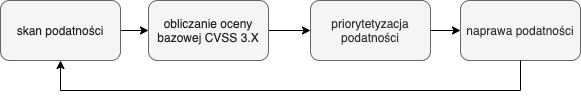
\includegraphics[width=.9\textwidth]{Chapters/Wstep/vm-models/vm-model-cvss3.png}
\caption{Model przepływu informacji w procesie zarządzania podatnościami z wykorzystaniem oceny bazowej CVSS 3.x.}
\label{fig:chapter1:vm-model-cvss3}
\end{figure}

\bigbreak
Autorzy takich prac jak \cite{fruhwirth2009improving, wang2015vulnerability, gallon2010impact} zauważyli, że wskazane modele wykorzystujące ocenę bazową (Rysunek \ref{fig:chapter1:vm-model-cvss2}, \ref{fig:chapter1:vm-model-cvss3}) są niewystarczające i oprócz nich należy brać jeszcze pod uwagę kontekst organizacji w celu dokładniejszego oszacowania poziomu bezpieczeństwa. Dlatego w niniejszej pracy zaproponowano dwa modele procesu zarządzania podatnościami wykorzystujące ocenę środowiskową CVSS. Rysunek \ref{fig:chapter1:vm-model-cvss2e} i \ref{fig:chapter1:vm-model-cvss3e} przedstawiają modele, które dodatkowo pobierają informacje o wagach zasobów z przygotowanej wcześniej bazy zasobów IT, dzięki czemu wykonują reprioretyzacje podatności uwzględniając ocenę środowiskową, która pozwala na lepsze dopasowanie oceny podatności do kontekstu organizacji. Tym samym pozwalają na identyfikacje wszystkich istotnych podatności bezpieczeństwa infrastruktury teleinformatycznej. Model pierwszy (Rysunek \ref{fig:chapter1:vm-model-cvss3e}), wykorzystujący ocenę środowiskową CVSS 3.x, posiada takie same wady jak wcześniej wspominany model wykorzystujący ocenę bazową CVSS 3.x (Rysunek \ref{fig:chapter1:vm-model-cvss3}) dotyczący braku oceny dla wszystkich podatności, dlatego również nie jest w stanie spełnić wymagań stawianych przez proponowane metryki CIS. Natomiast dzięki zastosowaniu metod konwersji oceny bazowej CVSS 2.0 do CVSS 3.x, przedstawionych w \cite{Nowa2109Conversion, Nowak-cldd-2021} możliwe jest jego w pełni zastosowanie. Model drugi (Rysunek \ref{fig:chapter1:vm-model-cvss2e}) z wykorzystaniem oceny środowiskowej CVSS 2.0 nie może być rozpatrywany jako samodzielny, ponieważ wpływ parametru $TD$, służący do ustalania liczby systemów wrażliwych na daną podatność, będzie znacząco zaniżał oceny wszystkich wykrytych podatności, w związku z czym stworzy on złudne wrażenie bezpieczeństwa monitorowanej infrastruktury teleinformatycznej, czyniąc ją bardziej podatną na ataki hakerskie. W rozdziale czwartym oraz piątym przedstawiony zostanie wpływ priorytetyzacji podatności za pomocą przedstawionych modeli na proces zarządzania podatnościami w celu weryfikacji tezy przedstawionej w rozdziale \ref{sec:zakres-i-teza-pracy}.

\begin{figure}[!ht]
\centering
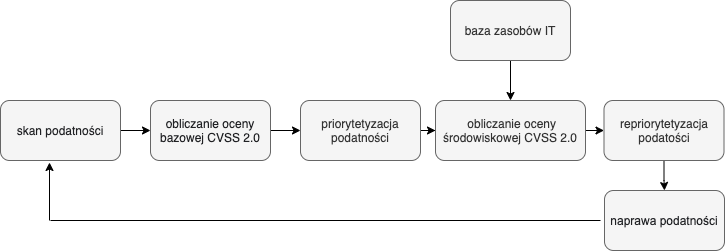
\includegraphics[width=.9\textwidth]{Chapters/Wstep/vm-models/vm-model-cvss-e-2.png}
\caption{Model przepływu informacji w procesie zarządzania podatnościami z wykorzystaniem oceny środowiskowej CVSS 2.0.}
\label{fig:chapter1:vm-model-cvss2e}
\end{figure}

\begin{figure}[!ht]
\centering
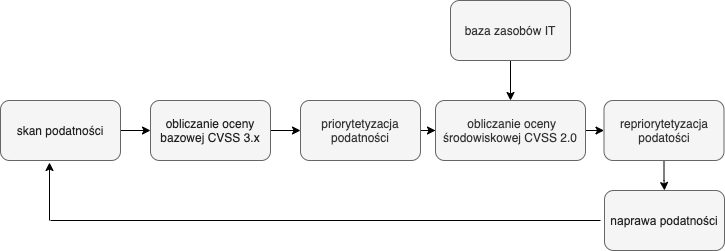
\includegraphics[width=.9\textwidth]{Chapters/Wstep/vm-models/vm-model-cvss-e-3.png}
\caption{Model przepływu informacji w procesie zarządzania podatnościami z wykorzystaniem oceny środowiskowej CVSS 3.x.}
\label{fig:chapter1:vm-model-cvss3e}
\end{figure}

\bigbreak
Kolejną ważną cechą opracowaną w niniejszej pracy jest również rozwiązanie problemu skalowalności. Pozwala to na łatwe dopasowanie narzędzia do rosnącej ilości napływających danych. Zgodnie z wynikami i dyskusjami przedstawionymi w dostępnej literaturze istotnym elementem zarządzania dużymi zbiorami danych jest ich cykl życia. W \cite{el2017data} autorzy przeanalizowali kilkanaście różnych cykli życia danych i ich faz, dążąc do znalezienia tych, które „czynią dane inteligentnymi, a tym samym ułatwiają zarządzanie nimi w kontekście Big Data”. „Inteligentny” oznacza wspomnianą wcześniej wiedzę uzyskaną z dużego i początkowo niestrukturyzowanego zbioru danych. Według \cite{lenk2015towards} „fazy składające się na cykl życia danych w kontekście Big Data są bardzo złożone. Każda faza jest uważana za jeden lub więcej złożonych, operacyjnych i niezależnych procesów, ale procesy te są ze sobą powiązane i sprawiają, że zarządzanie danymi jest bardziej elastyczne i inteligentne”. Zatem przedstawienie cyklu życia danych nie jest zadaniem trywialnym. W porównaniu z \cite{yadav2019patchrank, miura2007securerank, farris2018vulcon, chen2019vest} opracowane na potrzeby pracy doktorskiej oprogramowanie wykorzystuje informacje zebrane z bazy danych zasobów. W przeciwieństwie do \cite{fsecure2021, qualys2021, rapid72021, tenablevm2021} procedura ustalania priorytetów została szczegółowo opisana i dlatego może być analizowana przy użyciu standardu FIRST \cite{cvs2005specification, cvs2019specification}. Opracowane oprogramowanie jako produkt open source \cite{vmcgithub} charakteryzuje się przejrzystością stosowanych metod i technik.

\FloatBarrier
%%%%%%%%%%%%%%%%%%%%%%%%%%%%%%%%%%%%%%%%%%%%%%%%

%%%%%%%%%%%%%%%%%%%%%%%%%%%%%%%%%%%%%%%%%%%%%%%%
\section{Modele ewaluacji efektywności zarządzania podatnościami}
\label{sec:modele-ewaluacji-efektywnosci}
W celu ewaluacji efektywności modeli zarządzania podatnościami (Rysunek \ref{fig:chapter1:vm-model-cvss2}, \ref{fig:chapter1:vm-model-cvss3}, \ref{fig:chapter1:vm-model-cvss2e}, \ref{fig:chapter1:vm-model-cvss3e}) wykorzystano metrykę czasową zaprezentowaną w pracy \cite{farris2018vulcon}. Metryka mierzy szacunkową liczbę roboczogodzin wymaganych do poprawienia bezpieczeństwa infrastruktury. Autorzy pracy \cite{farris2018vulcon} przeprowadzili wywiad z inżynierami odpowiedzialnymi za naprawę podatności oraz podzielili je na trzy możliwe kategorie:
\begin{itemize}
    \item od 1 do 3 godzin (słabe metody szyfrowania, domyślne hasło lub poprawa konfiguracji),
    \item od 3 do 6 godzin (naprawa poprzez aktualizacje wersji oprogramowania),
    \item od 6 do 9 godzin (naprawa poprzez aktualizacje systemu operacyjnego).
\end{itemize}

Korzystając ze wspomnianych zakresów roboczogodzin, czas naprawy podatności ($T_{FIX}$) został podzielony na trzy podkategorie. Biorąc pod uwagę liczbę godzin potrzebnych do naprawy, $T_{FIX_{MAX}}$ reprezentuje maksymalną liczbę roboczogodzin wymaganą do naprawy jednej podatności (9 godzin), $T_{FIX_{AVERGE}}$ reprezentuje średnią liczbę roboczogodzin wymaganą do naprawienia jednej podatności (4.5 godziny) oraz $T_{FIX_{MIN}}$ reprezentuje minimalną liczbę roboczogodzin, która jest równa 1 godzinie. Następnie opracowano równania pozwalające oszacować liczbę roboczogodzin wymaganą do usunięcia istotnych podatności bezpieczeństwa infrastruktury teleinformatycznej. 

\bigbreak
Przy założeniu, że wszystkie podatności o klasyfikacji krytycznej ($X_C$), wysokiej ($X_H$) oraz średniej ($X_M$) muszą zostać naprawione przez administratorów, zakres wymaganej liczby roboczogodzin potrzebnych do usunięcia istotnych podatności bezpieczeństwa za pomocą proponowanych modeli zarządzania podatnościami można wyrazić za pomocą sumy iloczynów liczby podatności, które mają zostać naprawione oraz szacowanej liczby roboczogodzin, uwzględniającej czas trwania naprawy podatności. Dodatkowo w równaniu należy uwzględnić czas trwania skanowania ($T_S$). Dla modelu opartego o ocenę bazową CVSS 2.0 (Rysunek \ref{fig:chapter1:vm-model-cvss2}) równanie będzie miało następującą postać:
\begin{equation}
\label{eq:cvss2}
T_{Base2} = T_S + (T_{FIX} \cdot X_{H_\text{CVSS 2.0 Base}}) + (T_{FIX} \cdot X_{M_\text{CVSS 2.0 Base}})
\end{equation}
Gdzie $T_{FIX}$ to liczba roboczogodzin wymaganych do naprawy jednej podatności, $X_{H_\text{CVSS 2.0 Base}}$, $X_{M_\text{CVSS 2.0 Base}}$ to liczba podatności o odpowiednio wysokim i średnim poziomie krytyczności, zgodnie z oceną bazową CVSS 2.0.

\bigbreak
\begin{multline}
\label{eq:cvss3}
T_{Base3} = T_S + (T_{FIX} \cdot X_{C_\text{CVSS 3.x Base}}) + (T_{FIX} \cdot X_{H_\text{CVSS 3.x Base}}) + (T_{FIX} \cdot X_{M_\text{CVSS 3.x Base}}) 
\end{multline}
Gdzie $X_{C_\text{CVSS 3.x Base}}$ $X_{H_\text{CVSS 3.x Base}}$, $X_{M_\text{CVSS 3.x Base}}$ to liczba podatności o odpowiednio krytycznym, wysokim i średnim poziomie krytyczności zgodnie z oceną bazową CVSS 3.x.

\bigbreak
Ponieważ ocena bazowa CVSS jest oceną subiektywną, osoby zaangażowane w proces nie mają pewności, czy w kategorii o krytyczności niskiej ($X_L$) nie znajdują się podatności, które z punktu widzenia organizacji są istotne, czyli podatności o niedoszacowanej ocenie. Z tego względu administratorzy powinni naprawić wszystkie podatności, aby wyeliminować zaistniałe ryzyko nienaprawienia podatności z niedoszacowaną oceną \cite{gallon2010impact, li2015study}. Proponowane równanie dla modelu wykorzystującego ocenę bazową CVSS 2.0 (Rysunek \ref{fig:chapter1:vm-model-cvss2}) minimalizujące ryzyko nienaprawienia podatności niedoszacowanej będzie miało następującą postać:
\begin{equation}
\label{eq:cvss2prim}
T_{Base2'} = T_S + (T_{FIX} \cdot X_{H_\text{CVSS 2.0 Base}}) + (T_{FIX} \cdot X_{M_\text{CVSS 2.0 Base}}) + (T_{FIX} \cdot X_{L_\text{CVSS 2.0 Base}})
\end{equation}
Gdzie $T_{FIX}$ to liczba godzin pracy wymaganych do naprawy jednej podatności, $X_{H_\text{CVSS 2.0 Base}}$, $X_{M_\text{CVSS 2.0 Base}}$, $X_{ L_\text{CVSS 2.0 Base}}$ to liczba podatności o odpowiednio wysokim, średnim i niskim poziomie krytyczności, zgodnie z otrzymaną oceną bazową CVSS 2.0.

\bigbreak
Dla modelu zarządzania podatnościami opartego o ocenę bazową CVSS 3.x (Rysunek \ref{fig:chapter1:vm-model-cvss3}):
\begin{multline}
\label{eq:cvss3prim}
T_{Base3'} = T_S + (T_{FIX} \cdot X_{C_\text{CVSS 3.x Base}}) + (T_{FIX} \cdot X_{H_\text{CVSS 3.x Base}}) + (T_{FIX} \cdot X_{M_\text{CVSS 3.x Base}}) + \\
+ (T_{FIX} \cdot X_{L_\text{CVSS 3.x Base}})
\end{multline}
Gdzie $X_{C_\text{CVSS 3.x Base}}$ $X_{H_\text{CVSS 3.x Base}}$, $X_{M_\text{CVSS 3.x Base}}$, $X_ {L_\text{CVS 3.x Base}}$ to liczbą podatności o odpowiednio krytycznym, wysokim, średnim i niskim poziomie krytyczności zgodnie z otrzymaną oceną bazową CVSS 3.x.

\bigbreak
W przypadku modeli wykorzystujących ocenę środowiskową dodatkowo należy uwzględnić w równaniu czas ponownej priorytetyzacji za pomocą wytworzonego oprogramowania ($T_{VMC}$) oraz usunąć część równania odpowiedzialną za liczbę roboczogodzin potrzebnych do naprawy podatności niskich, ponieważ zakładamy, że ocena środowiskowa poprawnie wykonała prioretetyzacje z uwzględnieniem wymagań organizacji, w związku z czym wszystkie podatności zostały przypisane do odpowiadającej im kategorii, tym samym minimalizując ryzyko nienaprawienia niedoszacowanej oceny podatności. Dokładna możliwość zmiany oceny oraz kategorii podatności zostały szerzej omówione w rozdziale piątym. 

\bigbreak
Dla modelu środowiskowego CVSS 2.0 (Rysunek \ref{fig:chapter1:vm-model-cvss2e}) równanie przyjmie następującą postać:
\begin{equation}
\label{eq:cvss2e}
T_{Env2} = T_S + T_{VMC} + (T_{FIX} \cdot X_{H_\text{CVSS 2.0 Environmental}}) + (T_{FIX} \cdot X_{M_\text{CVSS 2.0 Environmental}})
\end{equation}
Gdzie $T_{VMC}$ jest czasem trwania ponownej priorytetyzacji wykonanej za pomocą opracowanego oprogramowania, $X_{H_\text{CVSS Environmental 2.0}}$ i $X_{M_\text{CVSS Environmental 2.0}}$ są odpowiednio liczbą podatności o wysokim i średnim poziomie krytyczności według oceny środowiskowej CVSS 2.0.

\bigbreak
Analogicznie dla przypadku modelu środowiskowego CVSS 3.x (Rysunek \ref{fig:chapter1:vm-model-cvss2e}):
\begin{multline}
\label{eq:cvss3e}
T_{Env3} = T_S + T_{VMC} + (T_{FIX} \cdot X_{C_\text{CVSS 3.x Environmental}}) + (T_{FIX} \cdot X_{H_\text{CVSS 3.x Environmental}}) + \\
+ (T_{FIX} \cdot X_{M_\text{CVSS 3.x Environmental}})
\end{multline}
Gdzie $X_{C_\text{CVSS 3.x Environmental}}$, $X_{H_\text{CVSS 3.x Environmental}}$ i $X_{M_\text{CVSS 3.x Environmental}}$ to odpowiednio liczba podatności o krytycznej, wysokiej i średniej krytyczności zgodnie z oceną środowiskową CVSS 3.x.

\bigbreak
Porównanie łącznej liczby roboczogodzin wymaganych do usunięcia podatności o kategorii krytycznej, wysokiej oraz średniej dla zaproponowanych modeli zarządzania podatnościami pozwoli określić bardziej wydajne rozwiązanie, a tym samym potwierdzić tezę przedstawioną w podrozdziale \ref{sec:zakres-i-teza-pracy}. Różnica liczby roboczogodzin między badanymi modelami zarządzania podatnościami określa potencjalne oszczędności, które można osiągnąć poprzez zmiany w mechanizmach priorytetyzacji podatności.

%%%%%%%%%%%%%%%%%%%%%%%%%%%%%%%%%%%%%%%%%%%%%%%%

%%%%%%%%%%%%%%%%%%%%%%%%%%%%%%%%%%%%%%%%%%%%%%%%
\section{Zakres i teza pracy}
\label{sec:zakres-i-teza-pracy}
Obecnie stosowane systemy priorytetyzacji podatności działają przy wykorzystaniu standardu CVSS 2.0 oceny krytyczności podatności. Ponadto skanery podatności obliczają jedynie ocenę bazową (ang. Base Score), a zatem nie uwzględniają wielu istotnych danych, które są potencjalnie dostępne dla operatora sieci teleinformatycznej. Takie podejście do zagadnienia priorytetyzacji podatności może skutkować błędnym zaszeregowaniem danej podatności. To z kolei może być przyczyną zwiększenia czasu pozostawania w systemie wielu podatności krytycznych, a tym samym zwiększa ryzyko naruszenia bezpieczeństwa zasobów.

\bigbreak
Teza pracy jest zatem następująca:

\bigbreak
\emph{Przy łącznym wykorzystaniu danych, które zawierają istotne informacje na temat infrastruktury sieci teleinformatycznej oraz danych pochodzących ze skanerów podatności możliwe jest w oparciu o otwarty standard CVSS (ang. Common Vulnerability Scoring System) stworzenie algorytmów zarządzania podatnościami o zwiększonej dokładności priorytetyzacji podatności bezpieczeństwa infrastruktury teleinformatycznej w porównaniu z rozwiązaniami opartymi jedynie na ocenie bazowej CVSS 2.0. Dzięki temu możliwe jest zmniejszenie liczby roboczogodzin potrzebnych do usunięcia istotnych podatności, a zatem także zmniejszenie czasu pozostawania tychże podatności w systemie.}

\bigbreak
Opracowany pakiet oprogramowania jest w zasadzie praktyczną realizacją Centrum Zarządzania Podatnościami (ang. Vulnerability Management Center, w skrócie VMC)  \cite{vmcgithub}. Zrealizowany w ramach tej pracy VMC pobiera informacje o zasobach IT z bazy inwentaryzacyjnej organizacji \cite{ralph} oraz podatności wykryte w monitorowanej infrastrukturze przy pomocy oprogramowania skanującego \cite{beale2004nessus, rahalkar2019openvas}. Następnie wykonuje ponowną priorytetyzację, wykorzystując standard CVSS 2.0 oraz 3.x, a zatem umożliwia realizację wszystkich rozważanych modeli procesu zarządzania podatnościami (Rysunki \ref{fig:chapter1:vm-model-cvss2}, \ref{fig:chapter1:vm-model-cvss3}, \ref{fig:chapter1:vm-model-cvss2e}, \ref{fig:chapter1:vm-model-cvss3e}).  Skuteczność metod priorytetyzacji podatności, które zaproponowano w tej pracy, została zweryfikowana na danych pozyskanych z rzeczywistych środowisk teleinformatycznych przy zastosowaniu metod przedstawionych w rozdziale \ref{sec:modele-ewaluacji-efektywnosci}. 

\bigbreak
Ponadto stworzone oprogramowanie VMC zostało wykorzystane w ramach realizacji projektu badawczego RegSoc \cite{regsoc}. Dokładny opis oprogramowania oraz sposobu implementacji zastosowanych metryk i reguł w projekcie RegSoc znajduje się w załącznikach Z3, Z4 i Z5.

%%%%%%%%%%%%%%%%%%%%%%%%%%%%%%%%%%%%%%%%%%%%%%%%

%%%%%%%%%%%%%%%%%%%%%%%%%%%%%%%%%%%%%%%%%%%%%%%%
\section{Układ pracy}
W rozdziale drugim opisano proponowane rozwiązania oraz architekturę stworzonego oprogramowania  wspomagającego proces zarządzania podatnościami w organizacjach \cite{rochford2008t, Gartner-2020}. Opracowane oprogramowanie korzysta z elementów infrastruktury, takich jak: skaner podatności \cite{beale2004nessus, rahalkar2019openvas}, publicznie dostępne bazy wiedzy o opublikowanych podatnościach \cite{booth2013national, exploitexploits}, systemy inwentaryzacji zasobów IT \cite{baron2010configuration} oraz systemy obsługi zgłoszeń \cite{thehive}. Dzięki normalizacji danych oraz przejrzystości interfejsu w przystępny sposób prezentuje w czasie rzeczywistym informacje dotyczące zagrożeń oraz alarmuje o odstępstwach od normy i anomaliach. Architektura rozwiązania umożliwia uruchomienie go w dowolnym środowisku w zależności od zapotrzebowania. Może to być chmura publiczna, chmura prywatna, serwer fizyczny lub maszyna wirtualna.

\bigbreak
Rozdział trzeci zawiera opis środowisk badawczych, w których przeprowadzono analizę zaproponowanych modeli zarządzania podatnościami. Wszystkie adresy IP wykorzystanych zasobów zostały zanonimizowane, ponieważ otrzymane dane pochodzą z rzeczywistych raportów oraz zawierają informacje poufne, które po ujawnieniu mogą wytworzyć dodatkowe zagrożenie dla organizacji, z których dane zostały pozyskane. Dodatkowo część administratorów dostarczyła informacje dotyczące ustawień środowiskowych z uwzględnieniem wag monitorowanych zasobów, dzięki czemu możliwe było odwzorowanie zachowania oprogramowania w warunkach laboratoryjnych.

\bigbreak
Rozdział czwartym poświęcony jest zbadaniu wpływu poszczególnych parametrów środowiskowych na ocenę bazową.  Uzyskane wyniki pozwoliły na wyciągnięcie wniosków dotyczących wykorzystania zmodyfikowanych równań przedstawionych w podrozdziale \ref{sec:modele-ewaluacji-efektywnosci} dotyczących szacowanej liczby roboczogodzin (Równania \ref{eq:cvss2e}, \ref{eq:cvss3e}).

\bigbreak
W rozdziale piąty omówione są najważniejsze wyniki analizy, które zostały przeprowadzone dla zaproponowanych modeli zarządzania podatnościami oraz opracowanego oprogramowania. Analiza została przeprowadzona na rzeczywistych zbiorach danych. Wykorzystane modele ewaluacji efektywności zarządzania podatnościami przedstawione w podrozdziale \ref{sec:modele-ewaluacji-efektywnosci} pozwoliły na zbadanie zmian zachodzących w priorytetyzacji podatności.

\bigbreak
Podsumowanie zawiera główne wnioski i opis dalszych kierunków badań, bibliografię oraz załączniki. W załącznikach zaś znajduje się dokumentacja dostarczona dla projektu Regionalne Centrum Bezpieczeństwa Cybernetycznego (RegSoc) zrealizowanego przez Wrocławskie Centrum Sieciowo-Super-komputerowe Politechniki Wrocławskiej \cite{regsoc}.